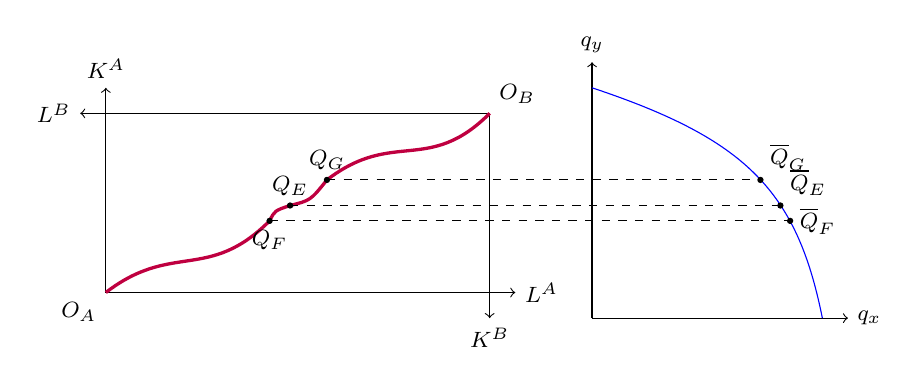
\begin{tikzpicture}[scale=0.65]
	% Caja de Edgeworth
		% Consumidor A
			\draw[->] (0.5,0.5) node[align=center, below left] {\footnotesize $O_A$} -- (0.5,4.5) node[align=center, above] {\footnotesize $K^A$};
			\draw[->] (0.5,0.5) -- (8.5,0.5) node[align=center, right] {\footnotesize $L^A$};
		
		%Consumidor B
			\draw[->] (8,4) node[align=center, above right] {\footnotesize $O_B$} -- (0,4) node[align=center, left] {\footnotesize $L^B$};
			\draw[->] (8,4) -- (8,0) node[align=center, below] {\footnotesize $K^B$};
		
		% Curva de contrato
			\draw  [purple, very thick] (0.5,0.5) ..controls (1.8,1.5) and (2.5,0.7) .. (3.7,1.9) .. controls (3.8,2.1) .. (4.1,2.2) .. controls (4.5,2.3) .. (4.82,2.7) ..controls (6.12,3.7) and (6.8,2.8) .. (8,4);
		
		% Punto
			\draw[black, fill=black] (4.82,2.7) circle[radius=0.05] node [above] {\footnotesize $Q_G$};
			\draw[black, fill=black] (4.1,2.2) circle[radius=0.05] node [above]  {\footnotesize $Q_E$};
			\draw[black, fill=black] (3.7,1.9) circle[radius=0.05] node [below]  {\footnotesize $Q_F$};
	
	% FPP
		% Ejes
			\draw[->] (10,0)-- (10,5) node[align=center, above] {\footnotesize $q_{y}$};
			\draw[->] (10,0) -- (15,0) node[align=center, right] {\footnotesize $q_{x}$};
		% Curva
			\draw [blue] (10,4.5) ..controls (13,3.5) and (14,2.5) .. (14.5,0);
		% Intersección
			\draw [dashed] (4.82,2.7) -- (13.29,2.7);
			\draw [dashed] (4.1,2.2) --  (13.68,2.2);
			\draw [dashed] (3.7,1.9) --  (13.87,1.9);
		% Puntos
			\draw[black, fill=black] (13.29,2.7) circle[radius=0.05] node [above right] {\footnotesize $\overline{Q}_G$};
			\draw[black, fill=black] (13.68,2.2) circle[radius=0.05] node [above right] {\footnotesize $\overline{Q}_E$};
			\draw[black, fill=black] (13.87,1.9) circle[radius=0.05] node [right] {\footnotesize $\overline{Q}_F$};
\end{tikzpicture}